\documentclass{article}

% Language setting
% Replace `english' with e.g. `spanish' to change the document language
\usepackage[english]{babel}

% Set page size and margins
% Replace `letterpaper' with `a4paper' for UK/EU standard size
\usepackage[letterpaper,top=2cm,bottom=2cm,left=3cm,right=3cm,marginparwidth=1.75cm]{geometry}

% Useful packages
\usepackage{amsmath}
\usepackage{graphicx}
\usepackage[colorlinks=true, allcolors=blue]{hyperref}

\title{BIOS 611 Final Project}
\author{Shuqi Zhang}

\begin{document}
\maketitle


\section{Introduction}
Global death counts due to cardiovascular disease (CVD) increased from 12.4 million in 1990 to 19.8 million in 2022 reflecting global population growth, aging and the contributions from preventable metabolic, environmental, and behavioral risks.  Heart attack is one of the life-threatening coronary events with sudden cardiac death and the most severe clinical presentation of coronary artery disease. Data science and machine learning can be used for diagnosing and predicting heart attack to save lives, improves health outcomes, and allocates healthcare resources efficiently. 

\section{Problem and Database Description}
The Kaggle dataset I selected is the “Heart Attack Risk Analysis Competition” which is ChatGPT generated. The competition aims to train a model to predict an individual is at high risk or low risk of a heart attack based on the input parameters including patient’s socio-demographics, clinical characteristics, lifestyle, and comorbidities. The outcome of this study is the occurrence of heart attack (1: Yes, 0: No). The other features include age, sex, country, continent where the patient resides, hemisphere where the patient resides, income, Body Mass Index (BMI), cholesterol, blood pressure, heart rate, triglycerides, smoking, alcohol consumption, exercise hours/week, diet, sedentary hours/day, physical activity/week, sleep/day, obesity, previous heart problems, medication use, stress level, diabetes, and family history. I mainly aim to solve the following two questions:

\subsection{To compare the model performance of Extra-trees classifier and Random Forest in predicting a participant had heart attack or not.}


\subsection{To identify the top 10 important features to prevent heart attack}

\section{Exploratory Data Analysis and Visualization}
Two datasets were provided by the competition. The training set includes 7,010 participants and the testing set includes 1,753 participants with undisclosed heart attack outcomes. In the training set, 30.23\% participants were female, with a mean age of 53.51 (SD=21.29). The BMI ranged from 18 to 40 Kg/m2 and the sleep duration ranged from 4 to 10 hours per day. The patients were from all around the world and very diversified, of whom 28.9\% were from Asia and 25.5\% were from Europe. Overall, 35.72\% participants had heart attack. 

\subsection{Visualization of participants' features}
The distributions of the input features by the heart attack outcome are presented in figures 1-4.

\begin{figure}
\centering
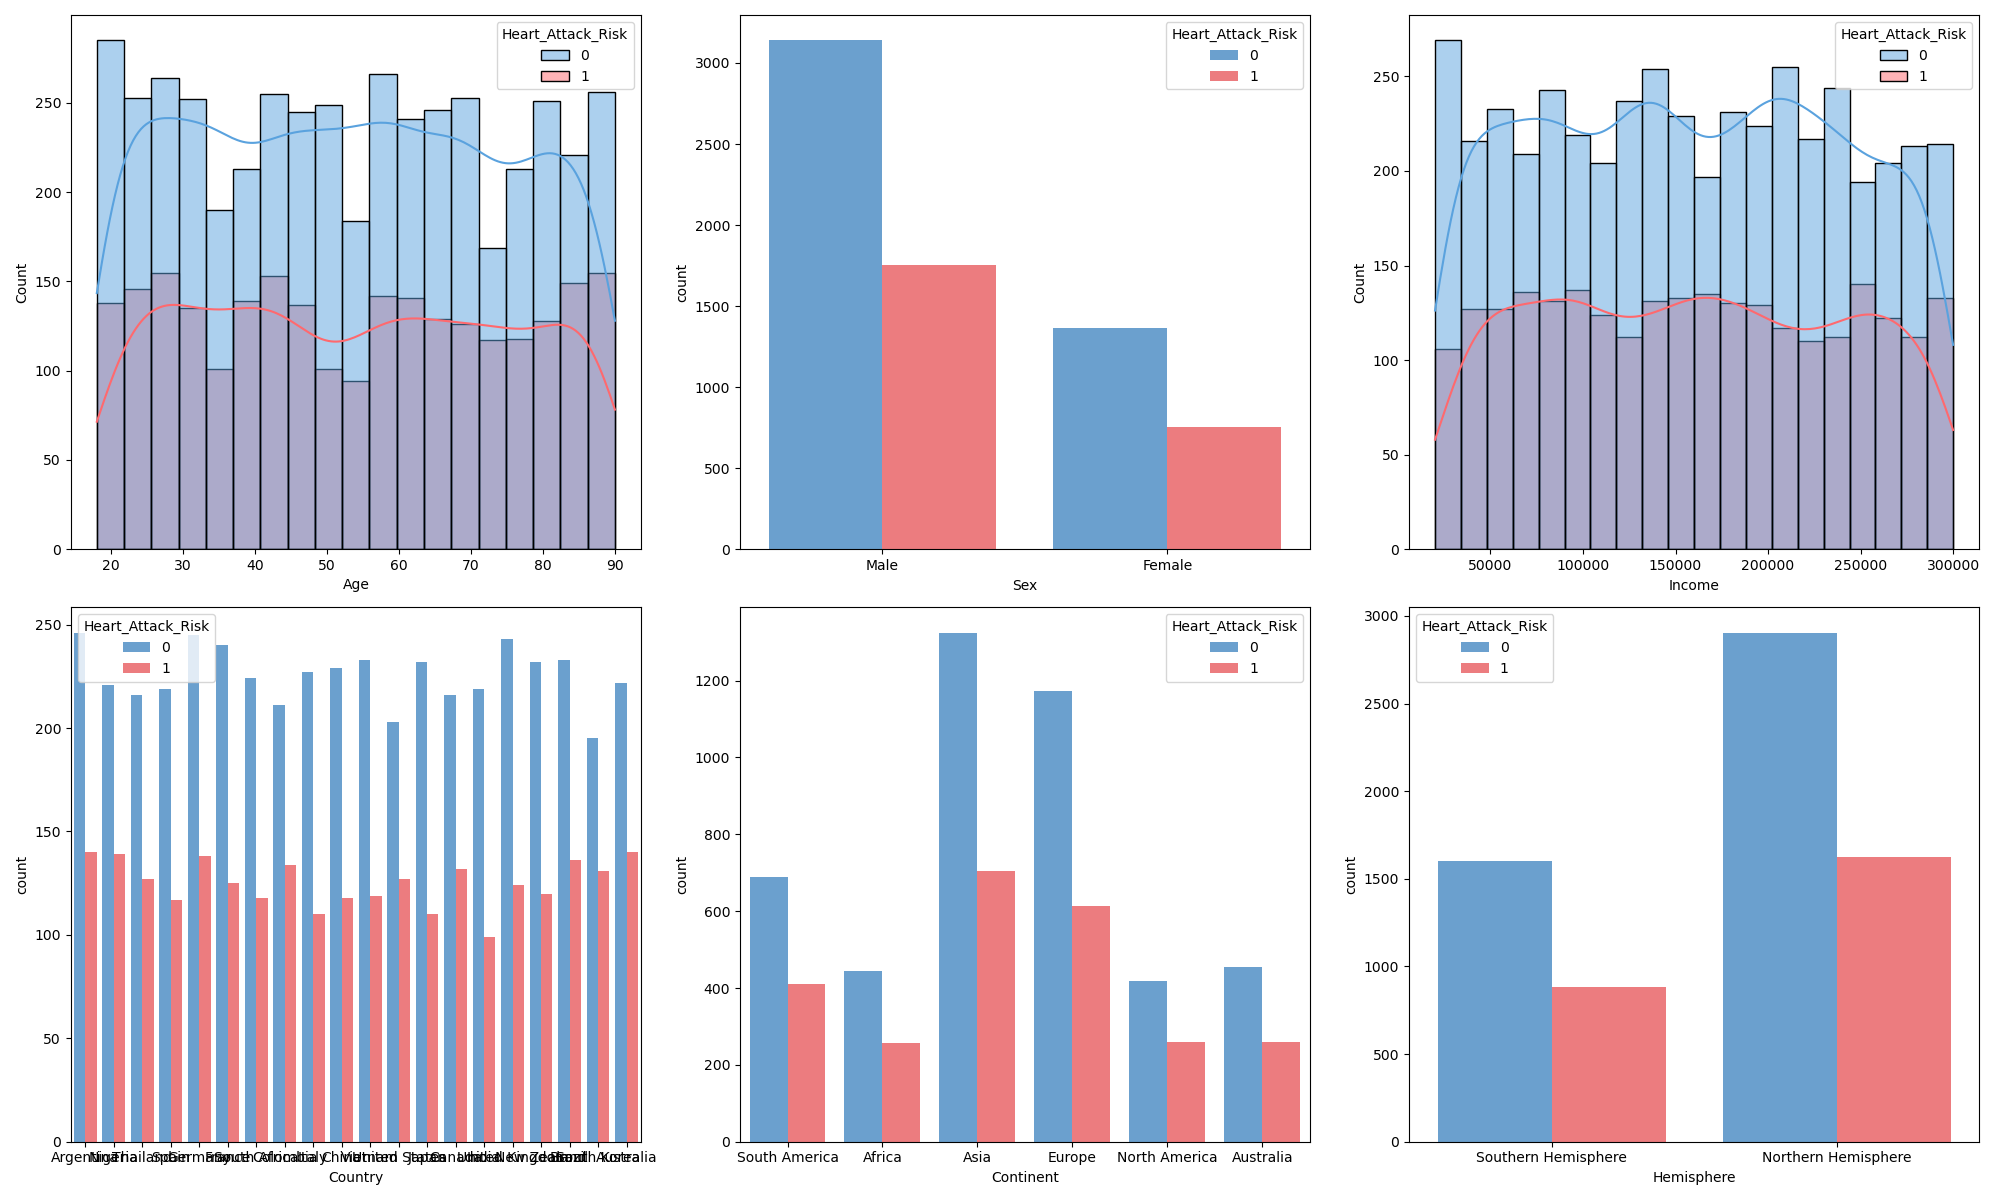
\includegraphics[width=1\linewidth]{figures/socio_demographics.png}
\caption{\label{fig:socio_demographics} Distributions of socio-demographic features by heart attack outcome.}
\end{figure}

\begin{figure}
\centering
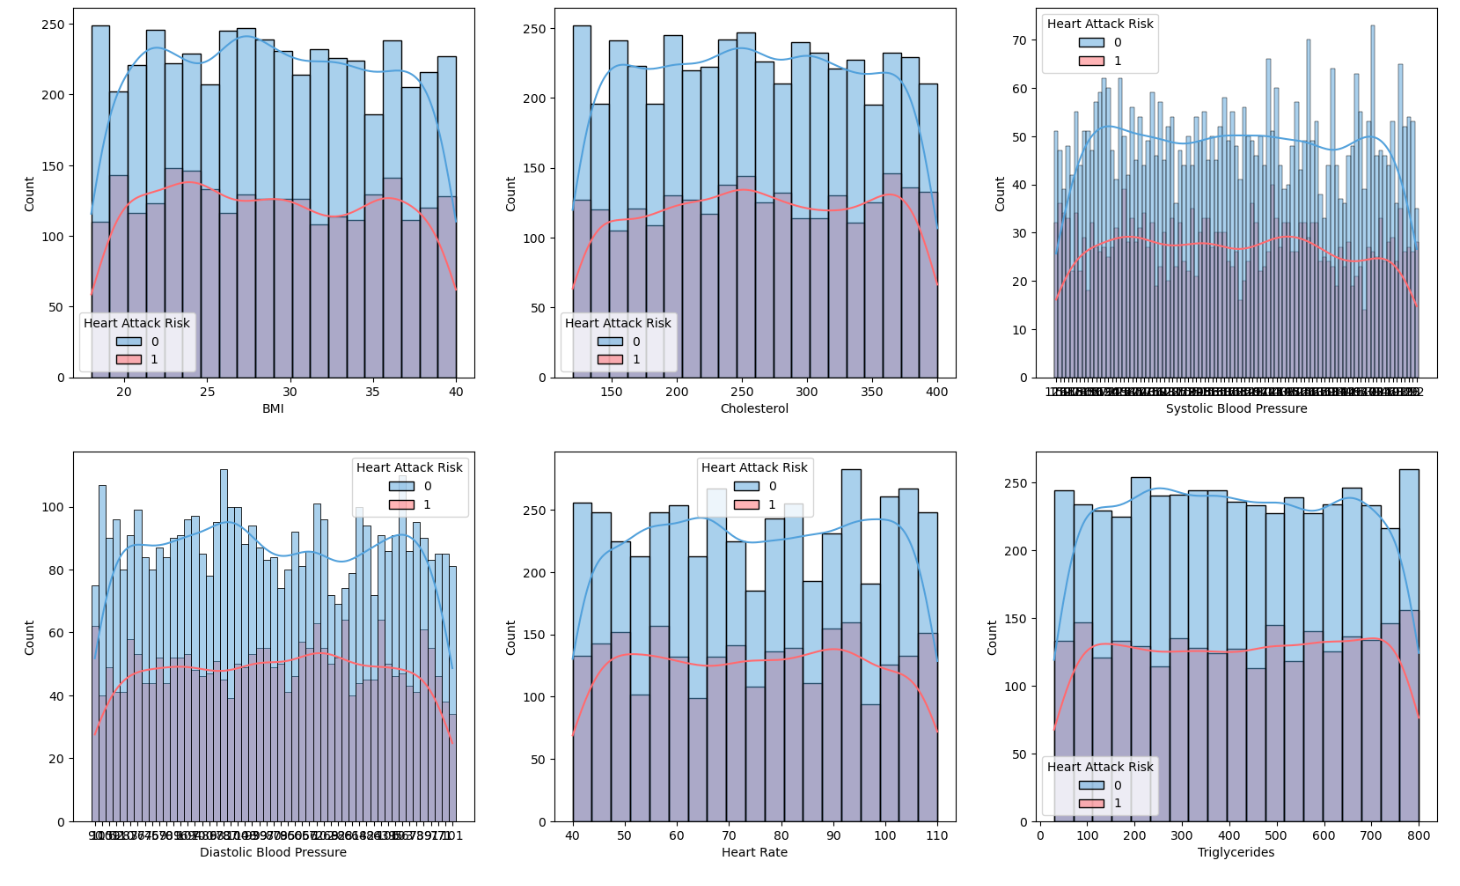
\includegraphics[width=1\linewidth]{figures/clinical_characteristics.png}
\caption{\label{fig:clinical_characteristics} Distributions of clinical characteristics by heart attack outcome.}
\end{figure}


\begin{figure}
\centering
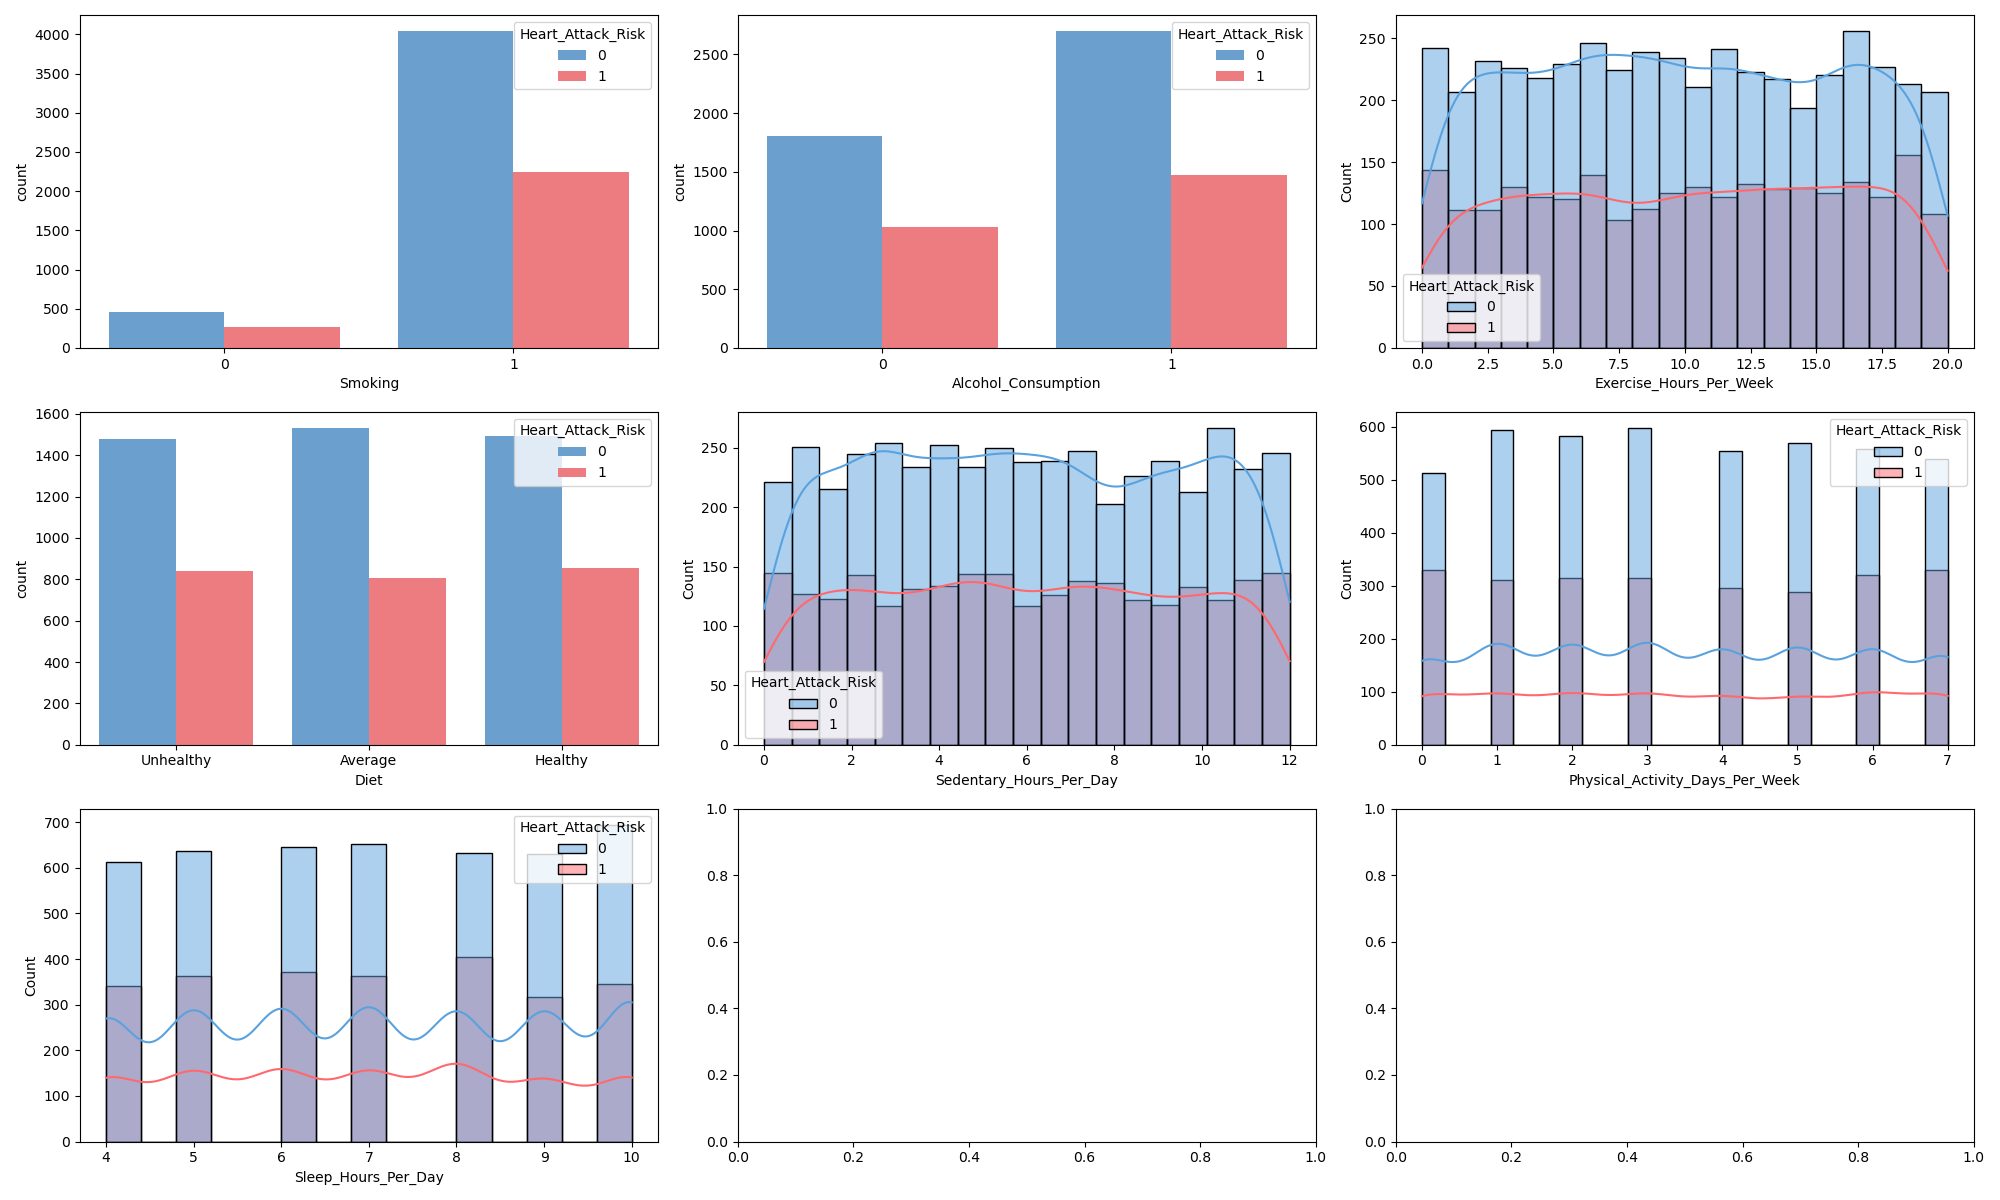
\includegraphics[width=1\linewidth]{figures/lifestyle_behaviors.png}
\caption{\label{fig:lifestyle_behaviors} Distributions of lifestyle behaviors by heart attack outcome.}
\end{figure}


\begin{figure}
\centering
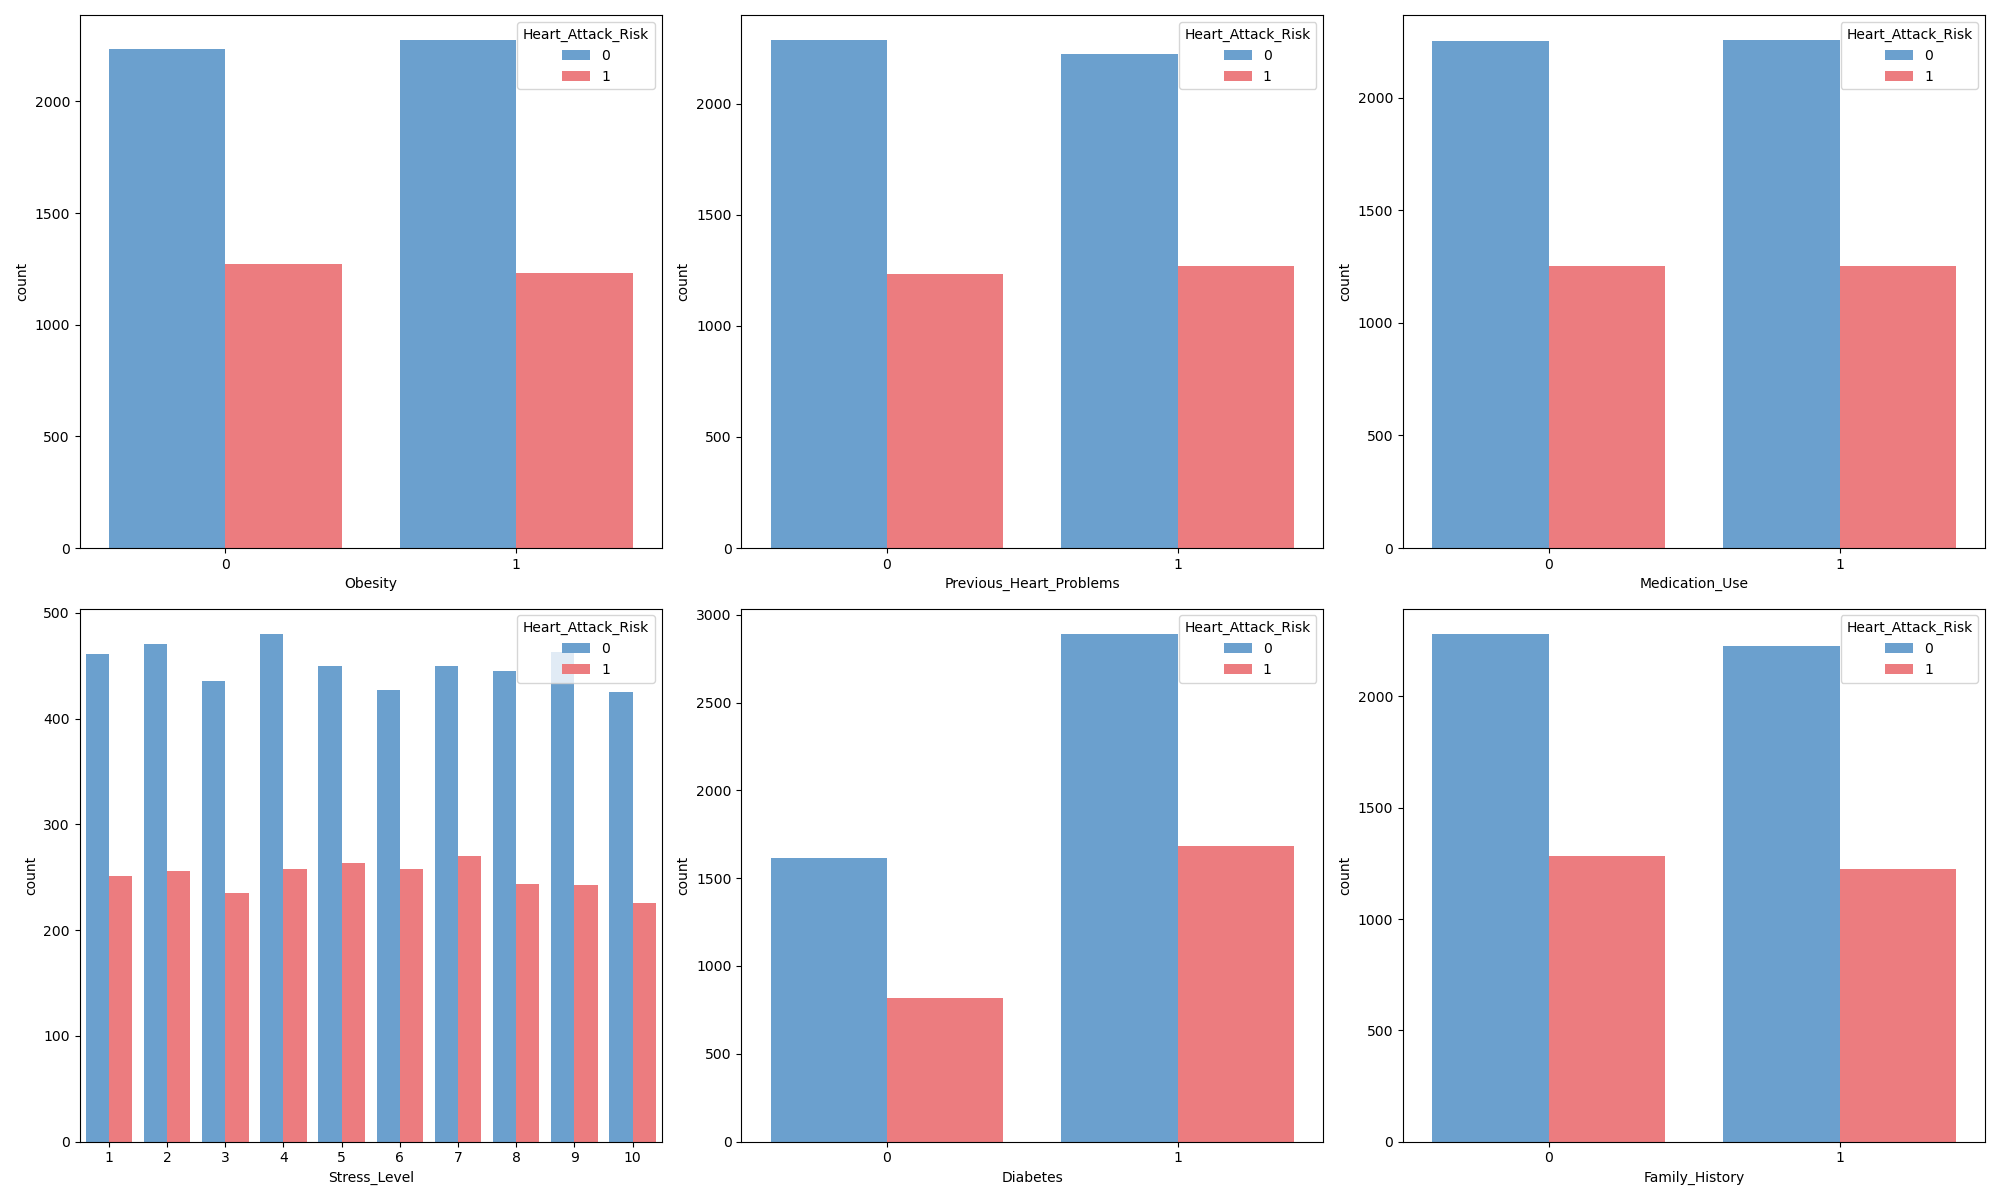
\includegraphics[width=1\linewidth]{figures/comorbidities.png}
\caption{\label{fig:comorbidities} Distributions of comorbidities by heart attack outcome.}
\end{figure}


\subsection{Correlation of participants' features}
From the heatmap of the correlation matrix of the features (figures 5), we found age and sex are highly associated with smoking.

\begin{figure}
\centering
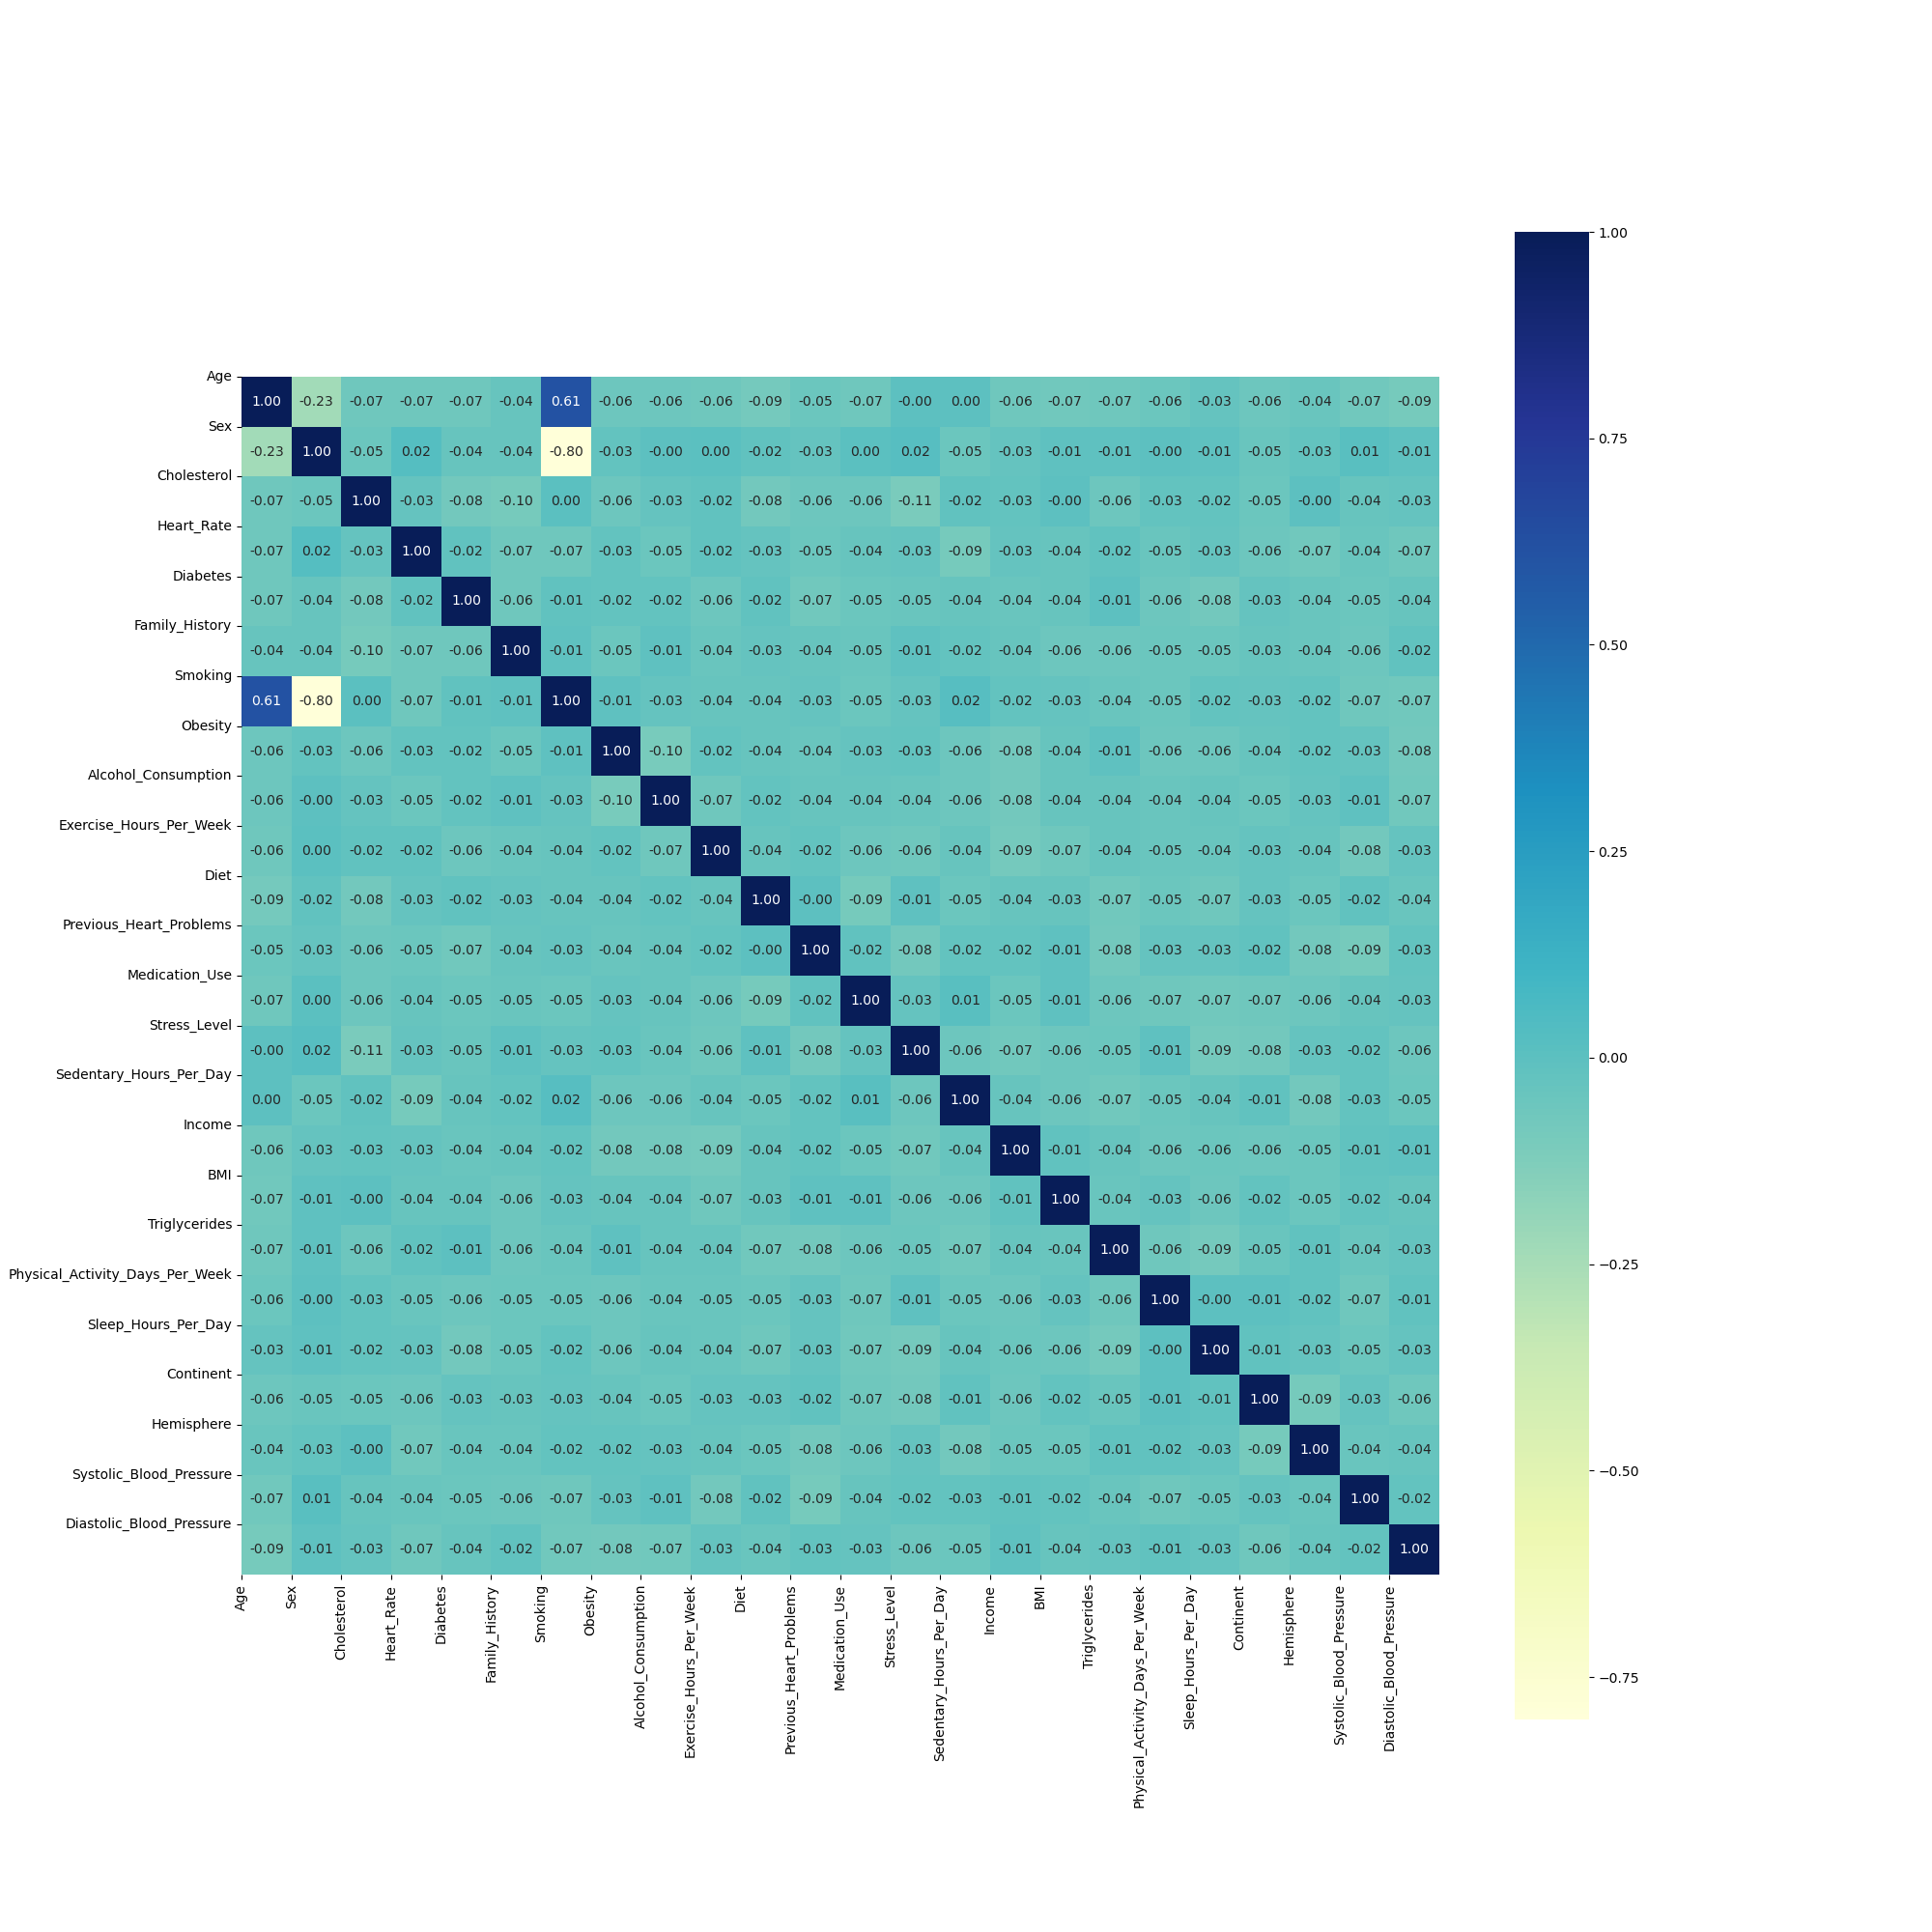
\includegraphics[width=1.3\linewidth]{figures/correlation_heatmap.png}
\caption{\label{fig:correlation_heatmap} Heatmap of the pairwise correlation matrix of the features.}
\end{figure}

\section{Data Preprocessing}
To prepare and process the data for modelling, I divided the combined blood pressure (e.g., 120/80 mmHg) into systolic blood pressure (120 mmHg) and diastolic blood pressure (80 mmHg). Then, I performed one-hot encoding and concerted all the categorical variables into a set of binary dummy variables.  All the features were standardized to reduce the models’ sensitivity to outlier. No missing value exists in the dataset.

\section{Models}
Two classification models were selected as candidate models. Some model characteristics and specified hyperparameters are described as fellows,\\
Extra Trees classifier can build multiple decision trees with high randomness, selecting random thresholds for each feature at each node, leading to reduced overfitting, improved generalization, and easy interpretability. I specified the number of trees in the Ext model as 20 to achieve a balance of the model performance and computational resources.\\
Random Forest is an ensemble learning approach constructing multiple decision trees with bootstrapped samples and random feature selection, boosting accuracy and resilience to overfitting, and suitable for large datasets with minimal tuning. The turning parameter I specified for the number of trees/bootstrapped samples was also 20 and for the number of predictors considered at each split was as the square root of the total number of features.

\subsection{Performance Metrics}
The model performance was mainly evaluated based on two metrics, accuracy score and F-1 score. The accuracy score is a metric to compare the number of predictions that match the true labels of the data. The F-1 score is a metric that considers both the precision and recall of the model to compute a single score that balances these two aspects.

\subsection{Cross Validation}
As common practice in Machine Learning, training dataset was preliminarily split into training set (80\%) and validation set (20\%). In addition, to test the robustness in estimating the performance of a ML model, I further evaluated the model performance through 10-fold cross-validation (CV). Average metrics and their standard deviations were estimated. The 10-fold CV can provide a more reliable assessment of model performance compared to one time train-test split

\section{Results}

\subsection{Model Performance}

\begin{table}[!ht]
    \centering
    \begin{tabular}{|l|l|l|l|l|}
    \hline
        ~ & ExtraTrees\_Accuracy & ExtraTrees\_F1 & RandomForest\_Accuracy & RandomForest\_F1  \\ \hline
        1 & 0.62 & 0.04 & 0.63 & 0.02  \\ \hline
        2 & 0.65 & 0.05 & 0.65 & 0.05  \\ \hline
        3 & 0.62 & 0.05 & 0.62 & 0.04  \\ \hline
        4 & 0.63 & 0.05 & 0.63 & 0.06  \\ \hline
        5 & 0.61 & 0.04 & 0.61 & 0.06  \\ \hline
        6 & 0.66 & 0.09 & 0.65 & 0.05  \\ \hline
        7 & 0.62 & 0.03 & 0.61 & 0.03  \\ \hline
        8 & 0.64 & 0.05 & 0.64 & 0.04  \\ \hline
        9 & 0.61 & 0.05 & 0.62 & 0.05  \\ \hline
        10 & 0.66 & 0.05 & 0.66 & 0.03  \\ \hline
        Average & 0.63 & 0.05 & 0.63 & 0.04 \\ \hline
    \end{tabular}
\end{table}


As we can observe from the table presenting the accuracy and F-1 score of Extra Trees and Random Forest obtained from 10-fold Cross-Validation, the two models have similar performance in accuracy and the Extra Trees did a litter better in F-1 score. Overall, both model had poor performance in predicting heart attack, since the ROC plots show they both got an AUC of around 0.5. The primary reason for the poor prediction performance is that the dataset was generated by AI, resulting in deviations from real-world data and a significant amount of noise.


\begin{figure}
\centering
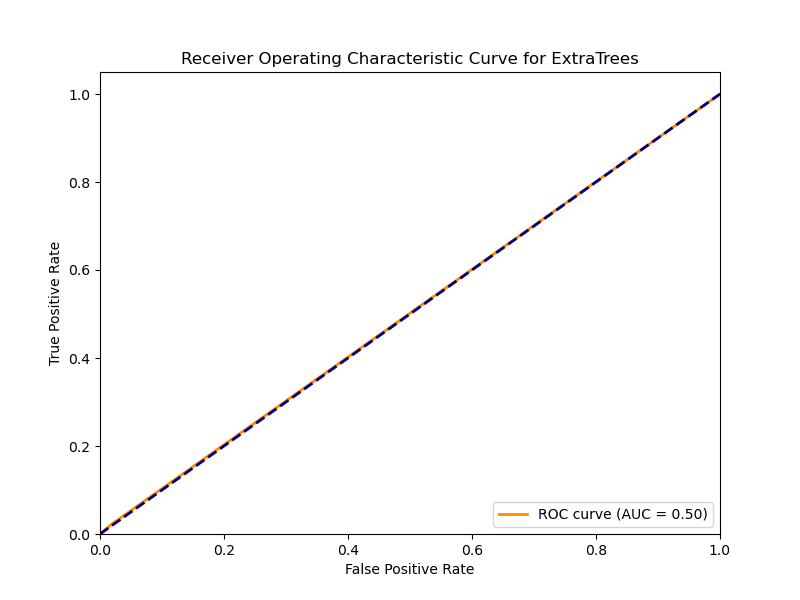
\includegraphics[width=0.6\linewidth]{figures/receiver_operating_characteristic_curve_for_extratrees.png}
\caption{\label{fig:ROC1} ROC plot for Extra Trees.}
\end{figure}


\begin{figure}
\centering
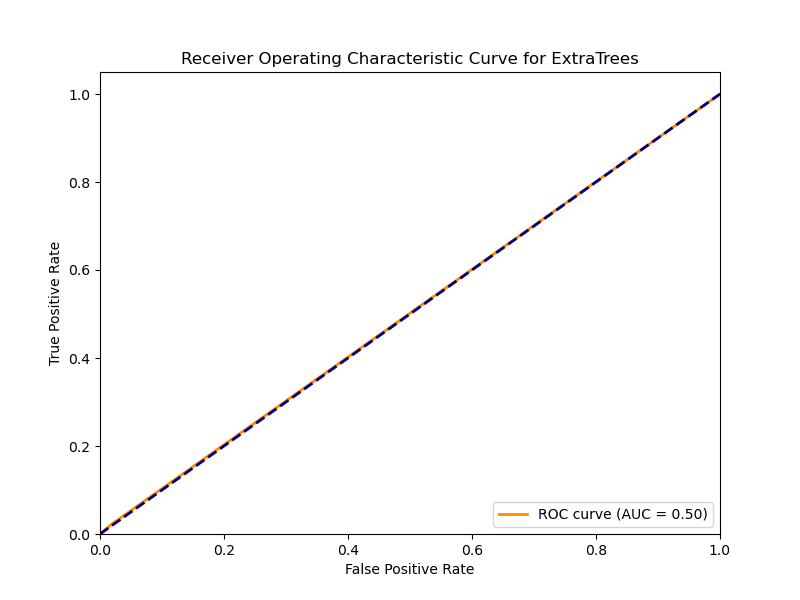
\includegraphics[width=0.6\linewidth]{figures/receiver_operating_characteristic_curve_for_extratrees.png}
\caption{\label{fig:ROC2} ROC plot for Random Forest.}
\end{figure}

\subsection{Feature importance}
Using the Extra Trees model and Random Forest model, we can identify 10 exactly same important features to answer the second question (see Figure 8-9). These features include age, sedentary hours per day, triglycerides, BMI, systolic blood pressure, exercise hours per week, cholesterol, heart rate, income, and diastolic blood pressure. However, the two methods gave slightly different ranks to the selected features. Except for age, We may intervene on those modifiable features to prevent population from getting heart attack.

\begin{figure}
\centering
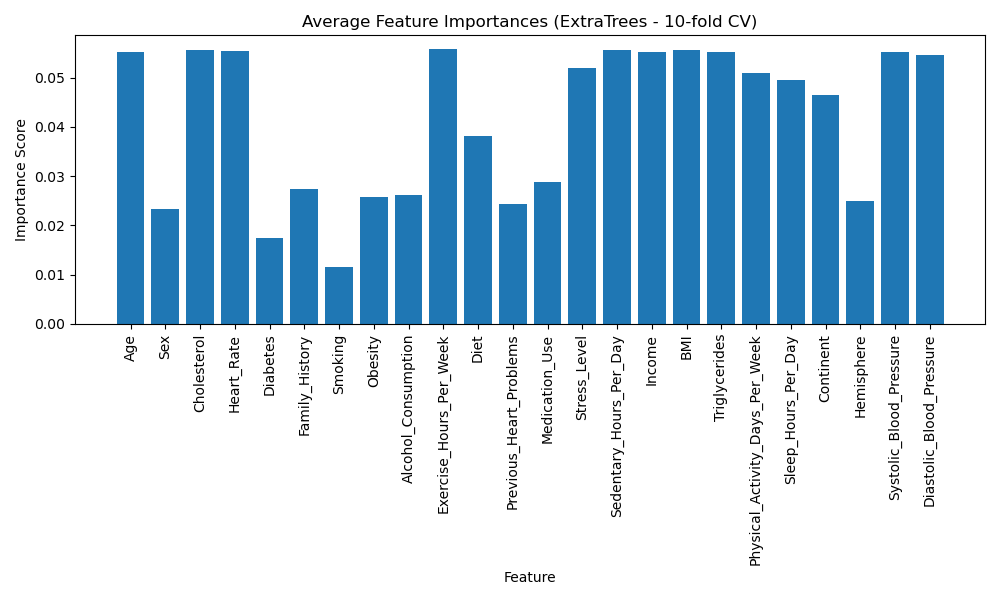
\includegraphics[width=1\linewidth]{figures/average_feature_importances_(extratrees_-_10-fold_cv).png}
\caption{\label{fig:FI_Ext} Feature importance identified from Extra Tree model.}
\end{figure}

\begin{figure}
\centering
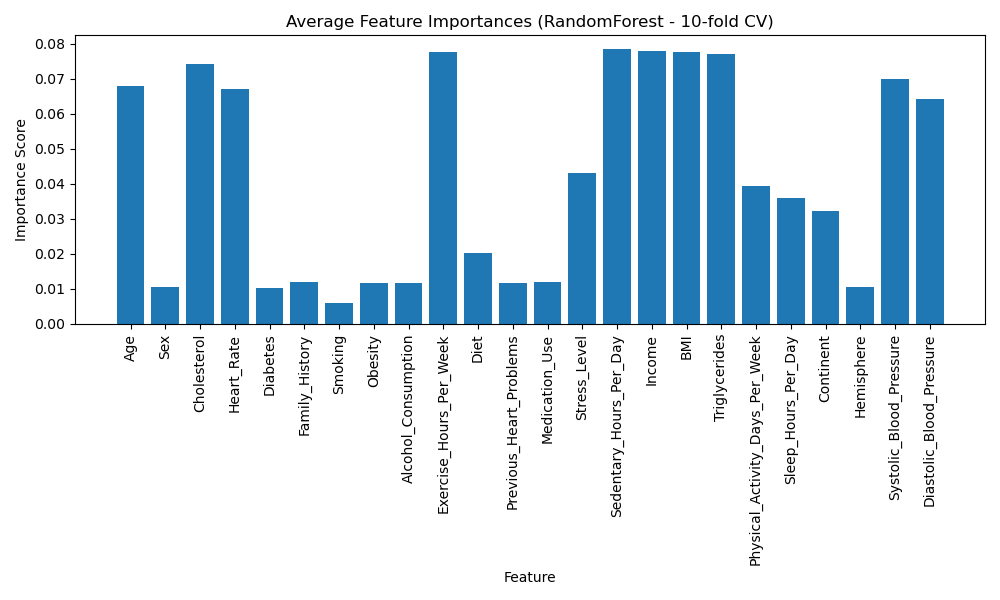
\includegraphics[width=1\linewidth]{figures/average_feature_importances_(randomforest_-_10-fold_cv).png}
\caption{\label{fig:FI_RF} Feature importance identified from Random Forest.}
\end{figure}


\end{document}